%%%%%%
%
% $Autor: Wings $
% $Datum: 2020-01-18 11:15:45Z $
% $Pfad: WuSt/Skript/Produktspezifikation/powerpoint/ImageProcessing.tex $
% $Version: 4620 $
%
%%%%%%

%todo WS: CNN heraus

\chapter{Processes for Knowledge Acquisition in Databases}

\section{Knowledge Discovery in Databases (KDD Process)}

Knowledge discovery in databases, or KDD for short, is the decisive step in the examination of data. There are various possibilities for knowledge discovery. However, in order to achieve the goal efficiently and systematically, a suitable process is of immanent importance. In this section, the KDD process is considered in detail. In this process, knowledge discovery is divided into several steps.  \cite{Dusing:2000}

\subsection{Application Areas}
The KDD process can basically be applied whenever large amounts of data are available from which knowledge can be extracted. The KDD process was presented in the article by Fayyad. \cite{Fayyad:1996}  There, astronomy, investment, marketing, fraud detection, manufacturing processes and telecommunications are given as examples on areas of application. But the KDD process is not limited to these areas. Thus, \cite{Maimon:2010} presents various applications in the fields of finance, medicine, detection of attacks on computer systems or customer relationship management. Although these examples exploit all elements of the KDD process in detail, application in these areas demonstrates the possible use of the entire KDD process with data mining as a core element. \cite{Pyo:2002} describes the application of the KDD process to data sets on tourist destinations, which can lead to insights into possibilities of increasing the attractiveness of individual destinations.

The literature mentioned shows the versatility of the KDD process. Basically, it can be used everywhere where sufficient data is available and a generalisation of certain structures is permissible. 


\subsection{Process Model}

One difficulty regarding the KDD process is that \glqq no general process model of Knowledge Discovery in Databases is currently available \grqq \cite{Dusing:2000}. There are several models that show the process steps starting from the data to the extracted knowledge.  One of the first and according to \cite{Kurgan:2006} the most cited model is the one according to Fayyad \cite{Fayyad:1996}. Therefore, it will be presented in the following. According to \cite{Kurgan:2006}, it is mainly the KDD process according to Fayyad and CRISP-DM that are also applied in the technical/engineering field, while many of the other models are rather aimed at areas in and around marketing. Therefore, both (Fayyad and CRISP-DM) will be described.  For this purpose, a generic model and such a model designed for application with edge computers will be presented.


\subsection{KDD-Prozess based on Fayyad}
On an abstract level, the field of KDD is concerned with the development of methods and techniques to \glqq make sense of data \grqq \cite{Fayyad:1996}. This requires going through several steps. The iterative nature of the process should be noted: Again and again, one can and must return to the previous steps and make corrections based on the knowledge gained. It may be necessary to obtain further data or introduce other pre-processing steps. \cite{Wrobel:1998}

The basic flow of the KDD process and the iteration loops included can be seen in Figure~\ref{KDDFayyad}.

\begin{figure}[H]
    \begin{center}
        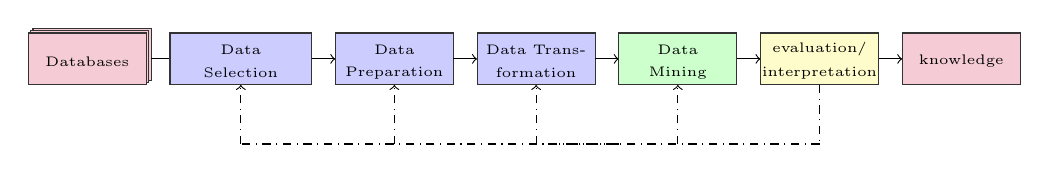
\begin{tikzpicture}[scale=0.6]
            \draw[draw, black!80, fill=blue!20!red!20] (-2.90,0.10) rectangle (-0.40,1.20);
            \draw[draw, black!80, fill=blue!20!red!20] (-2.95,0.05) rectangle (-.45,1.15);
            \draw[draw, black!80, fill=blue!20!red!20] (-3,0) rectangle (-0.5,1.1);
            \node (AMP) at (-1.75,0.5) {\tiny Databases};
            
            %\visible<2->
            {
                \draw[->] (-0.4,0.55)--(1.5,0.55);
                \draw[draw, black!80, fill=blue!20] (0,0) rectangle (3,1.1);
                \node (AMP) at (1.5,0.75) {\tiny Data};
                \node (AMP) at (1.5,0.25) {\tiny Selection};
            }
            
            %\visible<3->
            {
                \draw[->] (3,0.55)--(3.5,0.55);
                \draw[draw, black!80, fill=blue!20] (3.5,0) rectangle (6,1.1);
                \node (AMP) at (4.75,0.75) {\tiny Data};
                \node (AMP) at (4.75,0.25) {\tiny Preparation};
            }
            
            
            %\visible<4->
            {
                \draw[->] (6,0.55)--(6.5,0.55);
                \draw[draw, black!80, fill=blue!20] (6.5,0) rectangle (9,1.1);
                \node (AMP) at (7.75,0.75) {\tiny Data Trans-};
                \node (AMP) at (7.75,0.25) {\tiny formation};
            }
            
            %\visible<5->
            {
                \draw[dash dot,->] (10.75,-1.25)--(10.75,0);
                \draw[->] (9.0,0.55)--(9.5,0.55);
                \draw[draw, black!80, fill=green!20] (9.5,0) rectangle (12,1.1);
                \node (AMP) at (10.75,0.75) {\tiny Data};
                \node (AMP) at (10.75,0.25) {\tiny Mining};
            }
            
            {
                \draw[->] (12,0.55)--(12.5,0.55);
                \draw[draw, black!80, fill=yellow!20] (12.5,0) rectangle (15,1.1);
                \node (AMP) at (13.75,0.25) {\tiny interpretation};
                \node (AMP) at (13.75,0.75) {\tiny evaluation/};
            }
            
            \draw[->] (15,0.55)--(15.5,0.55);
            \draw[draw, black!80, fill=blue!20!red!20] (15.5,0) rectangle (18,1.1);
            \node (AMP) at (16.75,0.5) {\tiny knowledge};
            
            
            %\visible<8->
            {
                \draw[dash dot,-] (9.5,-1.25) -- (1.5,-1.25);
                \draw[dash dot,->] (1.5,-1.25)--(1.5,0);
            }
            
            %\visible<9->
            {
                \draw[dash dot,->] (4.75,-1.25)--(4.75,0);
                \draw[dash dot,->] (7.75,-1.25)--(7.75,0);
            }
            
            %\visible<2->
            {
                \draw[dash dot,-] (13.75,0)--(13.75,-1.25);
                \draw[dash dot,-] (13.75,-1.25) -- (8,-1.25);
                
            }
        \end{tikzpicture}
        \caption{KDD process according to \cite{Fayyad:1996} (own reduced representation based on \cite{Fayyad:1996})} 
        \label{KDDFayyad}
    \end{center}
\end{figure}



% \GRAPHICSC{1.0}{1.0}{BigData/KDD}



At the beginning of the KDD process there is always the available database from which the knowledge is to be gained. From this, the data to be used must be selected from one or more databases and the data must then be processed and prepared. Only then can the data be used for knowledge extraction with the help of data mining methods. After evaluation and possibly several runs through the various steps, the knowledge gained can finally be extracted and used in the application.

Fayyad further divides this process into nine sub-steps, some of which are not directly represented in Figure \ref{KDDFayyad}. These nine steps are described below.

\subsubsection{1. Domain Knowledge (Developing an Understanding of the Application Domain)}.

First, the domain of the application must be defined and understood. This includes the domain knowledge needed for the application to be able to perform the analysis in a way that leads to real added value. In addition, the precise objectives of the KDD process must be defined for the use case and the specific end user of the knowledge \cite{Fayyad:1996,Kurgan:2006}. This step forms the basis for making the decisions necessary in the next steps. 
necessary decisions in the next steps \cite{Maimon:2010}.

\subsubsection{2. Creating a Target Data Set}

Next, a data set or a subset of a data set is selected. Single or multiple variables can be selected to narrow down the data from which knowledge is to be extracted. \cite{Fayyad:1996} This involves determining what data is available and possibly obtaining any data that is still missing. It is important that all necessary information is included. Deciding which variables are necessary must be based on domain knowledge. After selecting the variables, as many representatives of the variables as possible should become available to the algorithm for a good model. On the other hand, the collection, storage and processing of larger data sets is more costly and many variables can also lead to results that are difficult to interpret. Therefore, the relevance of returning to steps that have already been carried out when gaining knowledge should already be seen in this step.\cite{Maimon:2010}

\subsubsection{3. Data Cleaning and Preprocessing}

This step aims to improve data reliability. This includes removing noise and outliers, but also dealing with missing data. If an attribute is not reliable enough, a data mining method can already be used at this point to improve the data.\cite{Maimon:2010} Time series information and known changes must also be taken into account. \cite{Kurgan:2006} Data cleaning and preparation is the most time-consuming step in the KDD process. Its share of the time to be spent on the KDD process is estimated by many sources to be about 60 \%.\cite{Kurgan:2006}

\subsubsection{4. Data Reduction and Transformation (Data Reduction and Projection)}.

To further improve the data, useful features are sought to represent the data \cite{Fayyad:1996}. Possible methods include dimensionality reduction and transformation. The implementation of this step will vary greatly depending on the application and domain. As in the previous steps, the most effective transformation may emerge during the KDD process \cite{Maimon:2010}. The importance of this step is made clearer by the application example in section~\ref{ExampleKDD}.

\subsubsection{5. Choosing the DM Task}

After the preparation of the data has been completed, a suitable data mining method is selected. Which method is suitable depends largely on the objectives defined in the first step \cite{Fayyad:1996}. A basic distinction is made between descriptive methods, which aim at interpreting and understanding the data, and predictive methods, which provide a behavioural model that is able to predict certain variables for previously unseen data. For this purpose, regressions can be used on the one hand, and classification methods such as decision trees, support vector machines or neural networks on the other. Some of these models can also be used for descriptive statements. \cite{Maimon:2010}

\subsubsection{6. Choosing the DM Algorithm}

In this step, the specific data mining algorithm to be used is selected. If, for example, it was decided in the previous step that a predictive method should be chosen, a choice must now be made between, for example, neural networks and decision trees, whereby the former provide more precise descriptions of the correlations, but the latter are easier to interpret. \cite{Maimon:2010}

\subsubsection{7. Data Mining}

In the seventh step, data mining is finally applied. Often data mining and KDD are used synonymously, but in fact data mining is a sub-step of the KDD process. \cite{Fayyad:1996}
This step may also have to be carried out several times, possibly even immediately one after the other, 
to optimise the hyperparameters. \cite{Maimon:2010}

\subsubsection{8. Interpreting the Results (Interpreting Mined Patterns)}

After the data mining has been successfully completed, the results are evaluated and interpreted. The visualisation of found patterns or models can be helpful for this. In this step, the influence of the data preparation steps is reflected on and possibly returned to. It must also be evaluated whether the model found is plausible and usable. \cite{Fayyad:1996,Maimon:2010}

\subsubsection{9. Applying the Results (Acting on Discovered Knowledge)}

The discovered knowledge can now be used. The product of this can be documentation or reports that record the knowledge obtained so that it can be used by interested parties. Furthermore, the extracted knowledge can be integrated into another system, e.g. in the form of a prediction model. By applying it under real conditions, e.g. with dynamic instead of static data, deficits can become apparent that still need to be reworked. \cite{Fayyad:1996,Maimon:2010}

\section{Generic Process Model}

Based on the models of Fayyad et al, Cabena et al, Cios et al and Anand \& Buchner and the CRISP-DM model, \cite{Kurgan:2006} describes a generic KDD model. This is structured very similarly to Fayyad's model described above and also runs through the steps iteratively. However, the steps are summarised differently, so that the model gets by with six instead of nine steps. 

\subsection{Application Domain Understanding}

As with Fayyad, the first step is to understand the application and objective as a prerequisite for the following steps.

\subsection{Understanding the Data (Data Understanding)}

The general understanding of the data corresponds roughly to the second step according to Fayyad. It involves looking at the available data set and identifying opportunities and problems.

\subsection{Data Preparation and Identification of DM Technology}

This step combines steps three to six according to Fayyad. This makes sense insofar as the type of data preparation and the data mining method to be applied influence each other and a clear separation is therefore difficult.


\subsection{Data Mining}

The data mining step as the core of the KDD process remains unchanged.

\subsection{Evaluation}

The generic model also emphasises the iterative nature of the KDD process. Therefore, an evaluation of the obtained results is indispensable.

\subsection{Knowledge Deployment (Knowledge Consolidation and Deployment)}

This step also hardly differs from the last process step according to Fayyad. The different models mainly differ in the way the discovered knowledge is used, which is due to the different application domains. While the models geared towards business applications mainly focus on reports and visualisation, the technical applications have a stronger emphasis on dynamic uses of created models.


\section{CRISP-DM} \label{CRISP}

While the first KDD models seem to be strongly oriented towards business applications, the CRoss-Industry Standard Process for Data Mining (CRISP-DM) is intended to be applicable to all industries and thus also to technical problems. CRISP-DM was developed in 1996 as part of a merger of the companies DaimlerChrysler, SPSS and NCR. The aim was to embed data mining in an industry-, tool- and application-independent process. The methodology is described with a hierarchical process model consisting of four abstraction levels: phases, generic tasks, specialised tasks and process instance. While the phases are always run through in the same way and the generic tasks are the same, which are described in more detail by the specialised tasks, the last level deals with the individual scope of application. \cite{Chapman:2000}

The CRISP-DM process model contains the life cycle of a data mining project as shown in Figure~\ref{CRISP-DM}. The phases shown are largely consistent with the phases described in the generic model. Ultimately, the KDD process is embedded in CRISP-DM. As mentioned, individual generic tasks are assigned to each phase, which must be processed in accordance with the specific task. In the phase \glqq Data preparation\grqq this includes data selection, cleansing, construction, integration and formatting. \cite{Chapman:2000}


\begin{figure}[H]
	\begin{center}
%		\includegraphics[width=0.6\textwidth]{kdd/CRISP-DM}
        
  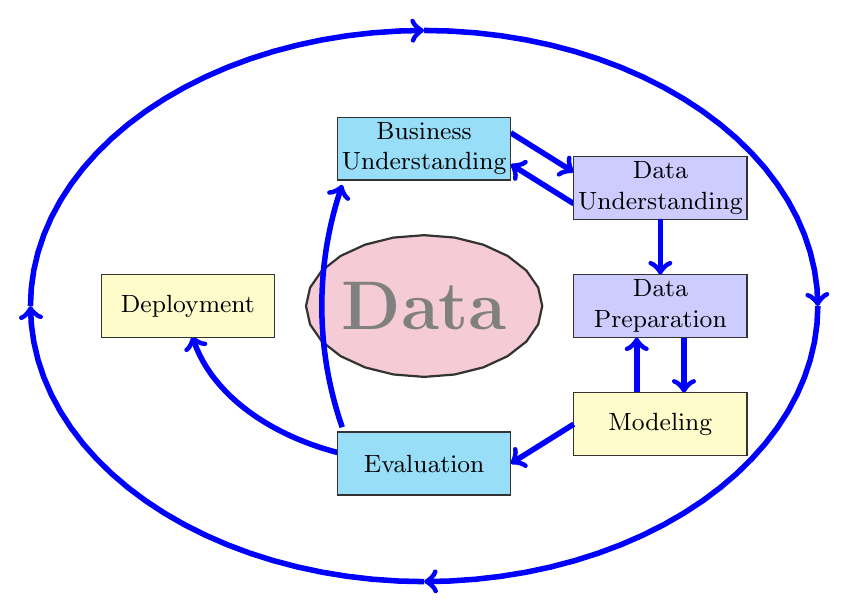
\begin{tikzpicture}
      
%      Cyan	#00FFFF	\definecolor{cyan}{rgb}{0.0, 1.0, 1.0}
    
    \draw [thick,domain=0:360,black!80, fill=blue!20!red!20] plot ({1.5*cos(\x)}, {0.9*sin(\x)});
    \node (D) at (0,0) {\Huge \textcolor{gray}{\textbf{Data}}};
    
    \draw [blue,line width = 2,domain=191:249,<-] plot ({3*cos(\x)}, {2*sin(\x)});

    \draw [blue,line width = 2,domain=160:200,<-] plot ({3+4.3*cos(\x)}, {4.5*sin(\x)});
    
    \draw [blue,line width = 2,->] (1.1, 2.2) -- (1.9,1.7);
    \draw [blue,line width = 2,<-] (1.1, 1.8) -- (1.9,1.3);
    \draw[black!80, fill=cyan!40] (-1.1,1.6) -- (1.1,1.6) -- (1.1,2.4) -- (-1.1,2.4) -- cycle;
    \node (BU) at (0,2) {\small \begin{tabular}{c} Business\\ Understanding \end{tabular}};
    
    
    \draw[black!80, fill=blue!20] (1.9,1.9) -- (4.1,1.9) -- (4.1,1.1) -- (1.9,1.1) -- cycle;
    \node (DP) at (3,1.5) {\small \begin{tabular}{c} Data\\ Understanding \end{tabular}};

    \draw [blue,line width = 2,->] (3, 1.1) -- (3,0.4);

    
    \draw[black!80, fill=blue!20] (1.9,0.4) -- (4.1,0.4) -- (4.1,-0.4) -- (1.9,-0.4) -- cycle;
    \node (DP) at (3,0) {\small \begin{tabular}{c} Data\\ Preparation \end{tabular}};

    \draw [blue,line width = 2,->] (3.3, -0.4) -- (3.3,-1.1);
    \draw [blue,line width = 2,<-] (2.7, -0.4) -- (2.7,-1.1);

    \draw[black!80, fill=yellow!20] (1.9,-1.9) -- (4.1,-1.9) -- (4.1,-1.1) -- (1.9,-1.1) -- cycle;
    \node (DP) at (3,-1.5) {\small Modeling};

    \draw [blue,line width = 2,<-] (1.1, -2) -- (1.9,-1.5);
    
    \draw[black!80, fill=cyan!40] (-1.1,-1.6) -- (1.1,-1.6) -- (1.1,-2.4) -- (-1.1,-2.4) -- cycle;
    \node (E) at (0,-2) {\small Evaluation};

    \draw[black!80, fill=yellow!20] (-1.9,0.4) -- (-4.1,0.4) -- (-4.1,-0.4) -- (-1.9,-0.4) -- cycle;
    \node (DP) at (-3,0) {\small \begin{tabular}{c} Deployment \end{tabular}};
    
    \draw [blue,line width = 2,domain=0:90,<-] plot ({5*cos(\x)}, {3.5*sin(\x)});
    \draw [blue,line width = 2,domain=90:180,<-] plot ({5*cos(\x)}, {3.5*sin(\x)});
    \draw [blue,line width = 2,domain=180:270,<-] plot ({5*cos(\x)}, {3.5*sin(\x)});
    \draw [blue,line width = 2,domain=270:360,<-] plot ({5*cos(\x)}, {3.5*sin(\x)});
  \end{tikzpicture}        
		\caption{Life cycle of a data mining project in CRISP-DM according to \cite{Chapman:2000}} 
		\label{CRISP-DM}
	\end{center}
\end{figure}

This model also emphasises the importance of returning to past phases during the process. In Figure~\ref{CRISP-DM} only the most important and frequent connections between the phases are shown. The outer circle represents the cyclical nature of the data mining process itself. \cite{Chapman:2000}

\section{Application-Oriented Process Models}

The models shown remain very abstract and little related to actual technical applications in a technical environment. In order to represent the actual processes when using different systems for knowledge generation and for use in the field, the following representations can be helpful.

For the description of artificial intelligence projects with the Jetson Nano, a modified KDD process model is assumed, which largely corresponds to the model according to Fayyad, but still contains some minor changes. This modified process model can be seen in Figure~\ref{KDDMod}.

\begin{figure}[H]
	\begin{center}
        
  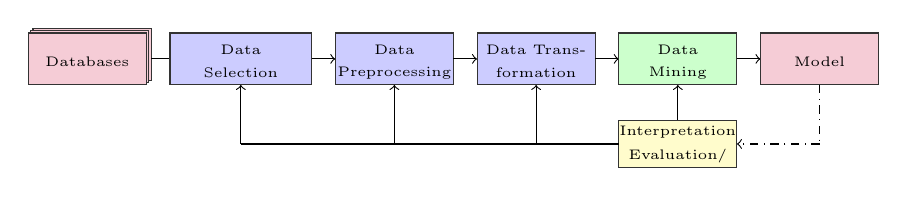
\begin{tikzpicture}[scale=0.6]
    \draw[draw, black!80, fill=blue!20!red!20]  (-2.90,0.10) rectangle (-0.40,1.20);
    \draw[draw, black!80, fill=blue!20!red!20]  (-2.95,0.05) rectangle (-.45,1.15);
    \draw[draw, black!80, fill=blue!20!red!20]  (-3,0) rectangle (-0.5,1.1);
    \node (AMP) at (-1.75,0.5) {\tiny Databases};
    
    %\visible<2->
    {
        \draw[->] (-0.4,0.55)--(1.5,0.55);
        \draw[draw, black!80, fill=blue!20]  (0,0) rectangle (3,1.1);
        \node (AMP) at (1.5,0.75) {\tiny Data};
        \node (AMP) at (1.5,0.25) {\tiny Selection};
    }
    
    %\visible<3->
    {
        \draw[->] (3,0.55)--(3.5,0.55);
        \draw[draw, black!80, fill=blue!20]  (3.5,0) rectangle (6,1.1);
        \node (AMP) at (4.75,0.75) {\tiny Data};
        \node (AMP) at (4.75,0.25) {\tiny Preprocessing};
    }
    
    
    %\visible<4->
    {
        \draw[->] (6,0.55)--(6.5,0.55);
        \draw[draw, black!80, fill=blue!20]  (6.5,0) rectangle (9,1.1);
        \node (AMP) at (7.75,0.75) {\tiny Data Trans-};
        \node (AMP) at (7.75,0.25) {\tiny formation};
    }
    
    %\visible<5->
    {
        \draw[->] (10.75,-1.25)--(10.75,0);
        \draw[->] (9.0,0.55)--(9.5,0.55);
        \draw[draw, black!80, fill=green!20]  (9.5,0) rectangle (12,1.1);
        \node (AMP) at (10.75,0.75) {\tiny Data};
        \node (AMP) at (10.75,0.25) {\tiny Mining};
    }
    
    {
%        \draw[->] (12,0.55)--(12.5,0.55);
        \draw[draw, black!80, fill=yellow!20]  (9.5,-1.75) rectangle (12,-0.75);
        \node (AMP) at (10.75,-1.0) {\tiny Interpretation};
        \node (AMP) at (10.75,-1.5) {\tiny Evaluation/};
    }
    
    \draw[->] (12,0.55)--(12.5,0.55);
    \draw[draw, black!80, fill=blue!20!red!20]  (12.5,0) rectangle (15,1.1);
    \node (AMP) at (13.75,0.5) {\tiny Model};
    
    
    %\visible<8->
    {
        \draw[-] (9.5,-1.25) -- (1.5,-1.25);
        \draw[->] (1.5,-1.25)--(1.5,0);
    }
    
    %\visible<9->
    {
        \draw[->] (4.75,-1.25)--(4.75,0);
        \draw[->] (7.75,-1.25)--(7.75,0);
    }
    
    %\visible<2->
    {
        \draw[dash dot,-] (13.75,0)--(13.75,-1.25);
        \draw[dash dot,->] (13.75,-1.25) -- (12,-1.25);
        
    }
  \end{tikzpicture}        
		\caption{Modified model of the KDD process based on the model according to \cite{Fayyad:1996}} 
		\label{KDDMod}
	\end{center}
\end{figure}

The lines marking the iterative loops are solid and not dashed to emphasise the absolute necessity of these iterative correction steps. However, the feedback from the model is shown dashed because in this process model it is assumed that the knowledge gained is used in the form of a model on an edge computer, here the Jetson Nano. This complicates direct feedback and corrections.

In Figure~\ref{KDDAnwendung} the distribution of the steps on different levels as well as localities and systems becomes clear. This illustration refers to the application in a production environment. It would be conceivable, for example, to create a system for process control that detects defective workpieces with the help of a camera. The database would be collected with this camera. The use of the data, including the steps explained in the previous sections, takes place in an office outside of production. However, the results found are used again in the control system in production, where they are exposed to new data. This new data can be added to the database(s) and possibly a feedback between the results in the field to a review and correction of the models taking place in the office can also be realised.

\begin{figure} [H]
\begin{center}   
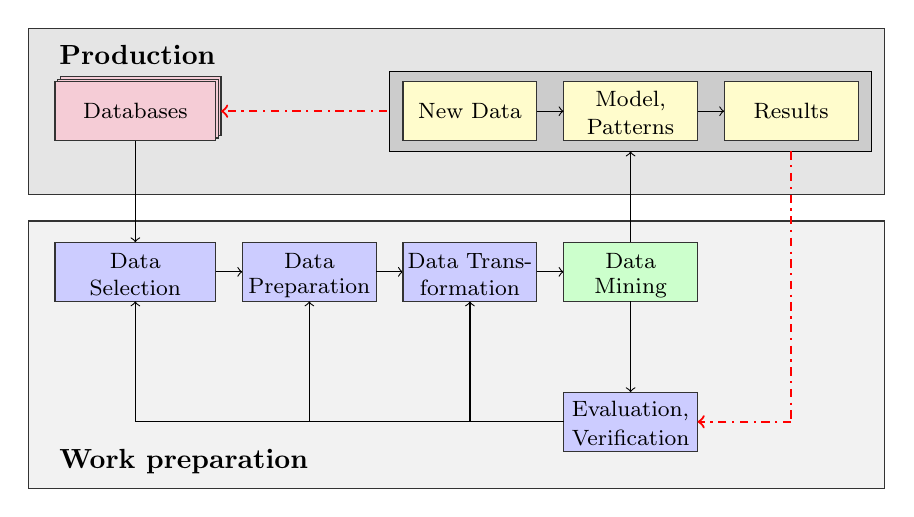
\begin{tikzpicture}[scale=0.68]
    \draw[draw, black!80, fill=black!10]  (-0.5,2) rectangle (15.5,5.1);
    
    \node[right] at (-0.1,4.6) {\textbf{Production}};
    
    \draw[draw, black!80, fill=black!5]  (-0.5,-3.5) rectangle (15.5,1.5);
    
    \node[right] at (-0.1,-3) {\textbf{Work preparation}};
    
    
    \draw[draw, black!80, fill=blue!20!red!20]  (0.10,3.10) rectangle (3.10,4.20);
    \draw[draw, black!80, fill=blue!20!red!20]  (0.05,3.05) rectangle (3.05,4.15);
    \draw[draw, black!80, fill=blue!20!red!20]  (0,3) rectangle (3,4.1);
    \node (AMP) at (1.5,3.55) {\footnotesize Databases};
    
    %\visible<2->
    {
        \draw[->] (1.5,3)--(1.5,1.1);
        \draw[draw, black!80, fill=blue!20]  (0,0) rectangle (3,1.1);
        \node (AMP) at (1.5,0.75) {\footnotesize Data};
        \node (AMP) at (1.5,0.25) {\footnotesize Selection};
    }
    
    %\visible<3->
    {
        \draw[->] (3,0.55)--(3.5,0.55);
        \draw[draw, black!80, fill=blue!20]  (3.5,0) rectangle (6,1.1);
        \node (AMP) at (4.75,0.75) {\footnotesize Data};
        \node (AMP) at (4.75,0.25) {\footnotesize Preparation};
    }
    
    
    %\visible<4->
    {
        \draw[->] (6,0.55)--(6.5,0.55);
        \draw[draw, black!80, fill=blue!20]  (6.5,0) rectangle (9,1.1);
        \node (AMP) at (7.75,0.75) {\footnotesize Data Trans-};
        \node (AMP) at (7.75,0.25) {\footnotesize formation};
    }
    
    %\visible<5->
    {
        \draw[->] (9.0,0.55)--(9.5,0.55);
        \draw[draw, black!80, fill=green!20]  (9.5,0) rectangle (12,1.1);
        \node (AMP) at (10.75,0.75) {\footnotesize Data};
        \node (AMP) at (10.75,0.25) {\footnotesize Mining};
    }
    
    %\visible<6->
    {
        \draw[fill=black!20] (6.25,2.8)--(6.25,4.3) -- (15.25,4.3) -- (15.25,2.8) -- cycle;
        
        \draw[->] (10.75,1.1)--(10.75,2.8);
        \draw[draw, black!80, fill=yellow!20]  (9.5,3) rectangle (12,4.1);
        \node (AMP) at (10.75,3.75) {\footnotesize Model,};
        \node (AMP) at (10.75,3.25) {\footnotesize Patterns};
    }
    
    {
        \draw[->] (9,3.55)--(9.5,3.55);
        \draw[draw, black!80, fill=yellow!20]  (6.5,3) rectangle (9,4.1);
        \node (AMP) at (7.75,3.55) {\footnotesize New Data};
    }
    
    {
        \draw[->] (12,3.55)--(12.5,3.55);
        \draw[draw, black!80, fill=yellow!20]  (12.5,3) rectangle (15,4.1);
        \node (AMP) at (13.75,3.55) {\footnotesize Results};
    }
    
    %\visible<7->
    {
        \draw[->] (10.75,0)--(10.75,-1.7);
        \draw[draw, black!80, fill=blue!20]  (9.5,-2.8) rectangle (12,-1.7);
        \node (AMP) at (10.75,-2.05) {\footnotesize Evaluation,};
        \node (AMP) at (10.75,-2.55) {\footnotesize Verification};
    }
    
    %\visible<8->
    {
        \draw[-] (9.5,-2.25) -- (1.5,-2.25);
        \draw[->] (1.5,-2.25)--(1.5,0);
    }
    
    %\visible<9->
    {
        \draw[->] (4.75,-2.25)--(4.75,0);
        \draw[->] (7.75,-2.25)--(7.75,0);
    }
    
    %\visible<2->
    {
        \draw[red, thick, dash dot,-] (13.75,2.8)--(13.75,-2.2);
        \draw[red,thick, dash dot,->] (13.75,-2.25) -- (12,-2.25);
        
        \draw[red,thick, dash dot,->] (6.2,3.55) -- (3.1,3.55);
    }
  \end{tikzpicture}
  \caption{KDD process in the industrial environment}\label{KDDAnwendung}
\end{center}
\end{figure}


\section{Role of the User}

Brachman and Anand \cite{Brachman:1994} criticise that the usual definitions of KDD are too focused on the resulting information and do not adequately reflect the complexity of the process. According to them, the role of the human being must be emphasised more, even if in the long run there is a move towards fully autonomous integrations of the KDD process. Front-end requirements must be recognised and reconciled, and data preparation, analysis and evaluation, as well as monitoring of the individual steps through visualisation, also require domain knowledge on the part of the user and his or her intervention. To support this, the authors recommend a corresponding working environment (Knowldege Discovery Support Environment) that allows easy data exchange between the different work steps as well as facilitates the reuse of already created structures. In addition, a system could support the user in the selection of suitable methodologies.


\section{KDD Process using the Example of Image Classification with an Edge Computer} \label{ExampleKDD}

To look at the process in relation to a tangible application, the development of an image classification with an Edge Computer as a KDD process will be highlighted as an example.

\subsection{Database}


As a data basis for an image classification, a sufficient number of images including their correct classification in terms of the application, the label, must be available. There are various image databases that are freely accessible, including ImageNet, MS-COCO and CIFAR-10, for example. Of course, only such databases come into question that contain objects and features that the model is to recognise later. \cite{Deng:2009,Deng:2012,Schutten:2016,Agarap:2018b} 

File formats and colour depth as well as the number of colour channels should also already be taken into account when searching for suitable databases, as a (lossless) transformation to the required file formats is not possible in every case or the database might contain less information than desired. Which file formats, colour depths and colour channels to use depends on the desired application, the training platform used and the algorithm used.

\subsection{Data Selection}

The images to be used can now be selected from the databases that have been identified, are available and can be used for the application. For example, a database could be used in its entirety, but only a part of such a database can be used or several databases can be combined. It is extremely important that all classes that are to be recognised are also present in the selected data. How many images are selected depends on the planned scope of the training and the test, which has a significant influence on the training time, but possibly also on the performance of the model obtained. 


\subsection{Data Preparation}

Data preprocessing is usually primarily concerned with data cleaning. This mainly includes the removal of outliers. In terms of images, these outliers are mainly noisy or poorly resolved images. These should be removed or processed with suitable algorithms. When using images from the well-known open-source image databases, such as ImageNet \cite{Deng:2009}, image quality should not be a problem.

Furthermore, the images must be converted into the format supported by the respective platform. It should be taken into account that compressed file formats cannot always be decompressed without loss.

\subsection{Data Transformation}

Finally, the images must be transformed into a representation that can be used in data mining. It may be necessary to adjust the colour depth per channel or the number of channels. An RGB image may need to be transformed into a greyscale image. It is also common to normalise the images, for example to mean 0 and standard deviation 1.

The algorithm chosen for the data mining phase also determines the input format of the data. Applied to images, this means which file format to use. In addition to the file format, however, the colour resolution determines the number of pixels. In this phase the images are adjusted accordingly.


\subsection{Data Mining}

In the data mining step, the actual model building takes place. First, the algorithm must be chosen or the architecture defined and the model built accordingly. If deep learning algorithms are used, the architecture must be defined. With the definition of the architecture, the hyperparameters are determined.  Then the algorithm can be trained with the selected images. During training, the weights are optimised. Their adjustment is done on the basis of the training images. After a given number of training images, the validation images are used to test the accuracy of the current model. After several epochs, i.e. several runs of all training images, the model can be tested.

\subsection{Evaluation/Verification}

In the first instance, the interpretation and evaluation of the trained model is done repeatedly during the training with the help of the validation data set. In the second instance, the model is tested directly after training with the help of the test images that are still unknown to the model. If the results are satisfactory, the model can be integrated into the application. In this instance, too, it is important to test the performance of the model in order to be able to draw conclusions and make corrections. In the dynamic application, other framework conditions prevail, so that drawing conclusions about necessary corrections in the previous steps may require great domain knowledge.

The interpretation of the found model is not trivial for neural networks, especially for complex networks like \ac{cnn}. It may not be possible to extract direct correlations that could be transferred to other applications.


\subsection{Model}

The trained model can finally be integrated into the intended application. While the data preparation and training take place on a computer that is generally equipped with high computing power, the model is intended to be used on an edge computer. For example, real-time object recognition could be performed with a camera connected to the Edge Computer based on the training with the static images. Transferring the model to the edge computer may require converting the model to a different format.


\section{Data Analysis and Data Mining Methods at a Glance}

The following is an overview of some data mining techniques.

\subsection{Definition Data Analysis}


Data analysis attempts to extract information from large amounts of data with the help of statistical methods and to visualise it afterwards. The complex field of data analysis can be divided into the areas of descriptive, inferential, exploratory and confirmatory data analysis. In descriptive data analysis, the information of the individual data, which was taken from a total survey, for example, is condensed and presented in such a way that the essentials become clear. If only the data of a sample survey (partial survey) is the basis, the focus of the data analysis rests on the transfer of the sample findings to the population. This is referred to as inferential data analysis. Explorative data analysis is concerned with processing the available amount of data in such a way that structures in the data as well as correlations between them can be revealed and highlighted to a particular degree. In contrast, the aim of confirmatory data analysis is to verify correlations.

\subsection{Statistical Data Analysis}

Statistical data analysis usually begins with calculations of the mean and standard deviation (or variance). It also involves checking the data for normal distribution.

\subsubsection{Hypothesis Test}

For the application of the hypothesis test, two hypotheses are always formulated: a null hypothesis $H_0$, which mostly implies that the presumed data structure does not exist, and the alternative hypothesis $H_1$ or $H_A$, which mostly implies that the presumed data structure exists. The hypothesis test refers to the assumption of a true null hypothesis \cite{Akremi:2011}. It must be proven that the null hypothesis is false. First, values such as the T-value ("The T-value is the quotient of the arithmetic mean of the differences between two variables being compared and the estimate of the standard error for this mean in the population." \cite{Akremi:2011}) or the F-value is calculated. These values are compared with a critical value adjusted to the situation. If this calculated value is smaller than the critical value, the null hypothesis is considered true. In this case, the P-value, i.e. the probability with which the result related to the null hypothesis occurs, is also only slightly smaller than 0.05. If, on the other hand, the P-value is very small, the null hypothesis is rejected. It is considered relatively certain that the null hypothesis is false; however, it is not known which hypothesis is correct. Conversely, if the null hypothesis is not rejected, it cannot be concluded that it is correct \cite{Akremi:2011}. In this case, the result cannot be interpreted.

\subsubsection{Normal Distribution, P-Test, T-Test}

The P-value (significance value) indicates how extreme the value of the test statistic calculated on the basis of the data collected is. It also indicates how likely it is to obtain such a sample result or an even more extreme one if the null hypothesis is true. Since the value is a probability value, it takes on values between zero and one. The P-value therefore indicates how extreme the result is: the smaller the P-value, the more the result speaks against the null hypothesis. Usually, a significance level $\alpha$ is set before the test and the null hypothesis is then rejected if the P-value is less than or equal to $\alpha$ \cite{Akremi:2011}. In order to be able to make decisions whether the null hypothesis should be rejected or retained, fixed limits have been established at about 5 \%, 1 \% or 0.1\%. If the null hypothesis is rejected, the result is called statistically significant. The size of the P-value does not indicate the size of the true effect.

The T-test refers to a group of hypothesis tests with a T-distributed test test size \cite{Akremi:2011}, but is often differentiated into one-sample T-test and two-sample T-test. The prerequisite for carrying out the T-test is the normal distribution of the population of data to be examined. Furthermore, there must be a sufficiently large sample size. If the data are not normally distributed, the T-test cannot be used and the principle of the U-test is applied. The one-sample T-test uses the mean value of a sample to test whether the mean value of the population differs from a given target value. The classic T-test (two-sample T-test), on the other hand, tests whether the mean values of two independent samples behave like the mean values of two populations. It is assumed that both samples come from populations with the same variance. The variance is the square of the standard deviation. The greater the variance, the flatter the normal distribution curve. If two sample sizes are compared, the weighted variance must also be determined. Here, the larger sample has the more decisive influence on the result.

\subsubsection{ANOVA (Analysis of Variance)}

\glqq Analysis of variance, usually called ANOVA in German, primarily looks for differences between groups and tests whether dividing the data into different groups reduces unexplained variability.\grqq \cite{Dormann:2013} Prerequisites for analysis of variance are normally distributed values in each group, approximate equality of standard deviations and independence of the measured values from each other. It is tested whether the mean values of several groups differ. In the simplest case, the null hypothesis is: The mean values of all groups are equal. Then the following alternative hypothesis results: Not all mean values are equal. The test variables of the procedure are used to test whether the variance between the groups is greater than the variance within the groups. This makes it possible to determine whether the grouping is meaningful or not, or whether the groups differ significantly or not. In its simplest form, the analysis of variance is an alternative to the T-test. The result is the same as with the T-test,\glqq because the results of a one-way analysis of variance (one-way ANOVA) and a T-test are identical if the two samples have the same variance.\grqq \cite{Dormann:2013}

\subsection{Overview of Data Mining Methods and Procedures}


Typical methods of data mining are:

\begin{itemize}
    \item cluster analysis: grouping of objects based on similarities,
    \item classification: elements are assigned to existing classes,
    \item association analysis: identification of correlations and dependencies in the data,
    \item regression analysis: identification of relationships between variables,
    \item outlier detection: identification of unusual data sets,
    \item correlation analysis: examines the relationship between two variables,
    \item summary: transformation of the data set into a more compact description without significant loss of information.
\end{itemize}

\bigskip

Here, outlier detection as well as cluster analysis belong to the observation problems; classification and regression analysis belong to the prediction problems.


\subsubsection{Cluster Analysis \& Classification}

Cluster analysis is used to reveal similarity structures in large data sets with the aim of identifying new groups in the data. The similarity groups found can be graph-theoretical, hierarchical, partitioning or optimising. The objects assigned to a cluster should be as homogeneous as possible, the objects assigned to different clusters should be very heterogeneous \cite{Janssen.2007}. In addition, several characteristics can be used in parallel when forming clusters. The cluster analysis is carried out in the following steps.

At the beginning, each object is considered as a single cluster. Then, the two individual objects that are most similar to each other are merged. The union reduces the number of clusters by one. Afterwards, all distances of the individual objects are calculated again and the two objects with the smallest distance are combined into a new cluster. This could theoretically be repeated until all objects are united in a single cluster, a so-called megacluster. However, for the analysis of the data, it is much more significant to determine the clustering that seems to make the most sense. The cluster number is determined by looking at the variance within and between the groups. It is determined which clustering seems to make the most sense, as no termination condition is specified for the function itself. As a rule, different cluster divisions are advantageous.

Prerequisites for the application of cluster analysis are metrically scaled characteristics, which can simply be included in the analysis; ordinally and nominally scaled characteristics must be scaled as dummy variables \cite{Janssen.2007}. Characteristics that are scaled in different dimensions can lead to a bias in the results. These values must be standardised before carrying out a cluster analysis, for example by a Z-transformation \cite{Janssen.2007}. Furthermore, the characteristics should not correlate with each other.

The distance between two individual objects is determined by the distance measure. The larger the measure, the more dissimilar the objects are. The various cluster methods \cite{Janssen.2007} are used to determine the distance between two clusters or a cluster and a single object. Classification, on the other hand, assigns data to already existing groups.

\subsubsection{Association Analysis \& Regression Analysis}

\glqq Association analysis generates rules that describe the relationships between the elements (items) that occur in the records of a dataset.\grqq \cite{Gluchowski:2006} These dependencies are represented in the form If item $A$, then item $B$ or $A \rightarrow B$. An item is the expression of an item. An item is the expression of an attribute value of a data set. An example of a simple rule would be: If a customer buys beer, then 70 per cent of the time he will also buy chips. These relationships are not assumed as hypotheses, but are to be discovered from the data with the association analysis. Only after a conspicuous pattern has been found is it investigated whether it is really a dependency and, if so, association rules are established for it. The parameters of association rules are support, confidence and lift. The greater the support value, the more relevant the rule.

Regression analysis is the analytical procedure for calculating a regression in the form of a regression line or function. The regression indicates which directional linear relationship exists between two or more variables \cite{Gluchowski:2006}. The coefficient of determination (R²) expresses how well the regression line reflects the relationship between the independent and dependent variable. R² lies between 0 and 1, whereby the value R² = 1 would mean that every observed data point lies directly on the regression line. By determining a regression function, no statement can be made about the significance of a correlation. The significance of the regression is determined by the F-test.


At the beginning of the regression analysis is the preparation of the data. Missing data are omitted or filled in, data are transformed and the interactions (in linear regression) are taken into account. By means of mathematical procedures, a function f is determined so that the residuals e become minimal (residuals: difference between a regression line and the measured values \cite{Kaehler:2011}). Model validation, i.e. checking whether the model is a good description of the correlation, includes the

\begin{itemize}
    \item residual analysis,
    \item overfitting,
    \item examining the data for outliers and influential data points, and
    \item multicollinearity of the independent variables.
\end{itemize}	

\bigskip
The validated model can be used to forecast values of y given values of x. To estimate the uncertainty of the prediction, a confidence interval is often given in addition to the predicted y-value.


\subsubsection{Outlier Detection}

Outliers are measured values or findings that are inconsistent with the rest of the data, for example, by having unusual attribute values or not meeting expectations. Expectation is most often the range of dispersion around the expected value in which most measured values are found. \glqq Robust bounds for detecting outliers for many distribution types can also be derived based on quartiles and quartile distance.\grqq \cite{Sachs:2006} Values of exploratory studies that lie further than 1.5 times the quartile distance outside this interval are called outliers. Particularly high outliers are shown separately in the boxplot.

For example, the Local Outlier Factor procedure searches for objects that have a density that deviates significantly from their neighbours, then this is referred to as density-based outlier detection. Identified outliers are then usually verified manually and removed from the data set, as they can worsen the results of other procedures. Before deciding in favour of removing values, it is therefore still necessary to check in each case what data loss occurs when deleting or labelling the missing values. If the number of available data sets falls below the level necessary to proceed, the removal of the outliers should be avoided.

	
\subsubsection{Correlation Analysis}

An important task of data analysis is the analysis of the correlation between individual characteristics. The strength of the connection between two quantitative characteristics is called correlation in descriptive statistics and inferential statistics and can be differentiated into linear and non-linear correlation. In multivariate data sets, the correlation coefficient is additionally calculated for each pair of variables.\cite{Goettingen} \glqq For correlation analysis, mainly methods of classical, multivariate, robust and exploratory statistics are used, but also various non-linear regression methods whose approximation errors can be used as correlation measures.\grqq \cite{Runkler.2015} A prerequisite for performing correlation analysis is the normal distribution of the data under investigation.

\subsubsection{Summary as a Method of Data Mining}

By transforming a data set into a more compact description of its information, summarisation ensures a lossless representation of essential information. The summary can be textual, visual or combined.



%
%[1] Vgl. Akremi, L., Baur, N., Fromm, S. (Hrsg.), Datenanalyse mit SPSS für Fortgeschrittene 1 – Datenaufbereitung und uni- und bivariate Statistik, 3., überarbeitete und erweiterte Auflage, Springer Fachmedien, Wiesbaden, 2011, S. 247.
%[2] „Der T-Wert ergibt sich aus dem Quotienten des arithmetischen Mittels der Differenzen zwischen zwei zu vergleichenden Variablen und dem Schätzwert des Standardfehlers für dieses Mittel in der Grundgesamtheit.“ Zitiert aus Akremi, L., Baur, N., Fromm, S. (Hrsg.), 2011, S. 267.
%[3] Vgl. Akremi, L., Baur, N., Fromm, S. (Hrsg.), Datenanalyse mit SPSS für Fortgeschrittene 1 – Datenaufbereitung und uni- und bivariate Statistik, 3., überarbeitete und erweiterte Auflage, Springer Fachmedien, Wiesbaden, 2011, S. 200.
%[4] Vgl. Akremi, L., Baur, N., Fromm, S. (Hrsg.), Datenanalyse mit SPSS für Fortgeschrittene 1 – Datenaufbereitung und uni- und bivariate Statistik, 3., überarbeitete und erweiterte Auflage, Springer Fachmedien, Wiesbaden, 2011, S. 203.
%[5] Vgl. Akremi, L., Baur, N., Fromm, S. (Hrsg.), Datenanalyse mit SPSS für Fortgeschrittene 1 – Datenaufbereitung und uni- und bivariate Statistik, 3., überarbeitete und erweiterte Auflage, Springer Fachmedien, Wiesbaden, 2011, S. 257.
%[6] Zitiert aus Dormann, C., Parametrische Statistik – Verteilungen, miximum likelihood und GLM in R, 2., überarbeitete und erweiterte Auflage, Springer-Verlag, Berlin, 2013, S. 199.
%[7] Zitiert aus Dormann, C., Parametrische Statistik – Verteilungen, miximum likelihood und GLM in R, 2., überarbeitete und erweiterte Auflage, Springer-Verlag, Berlin, 2013, S. 202.
%[8] Zitiert aus Hung, P. T., Data-Mining und KDD – ein Überblick, TU Dresden, 2009, S. 3.
%[9] Vgl. Hung, P. T., Data-Mining und KDD – ein Überblick, TU Dresden, 2009, S. 9.
%[10] Vgl. Queckbörner, S., Was ist Data Mining?, Technische Universität Kaiserslautern, o. J., S. 7.
%
%[11] Vgl. Böhm, Chr., Vorlesung „Knowledge Discovery in Databases“, Ludwig Maximilians Universität München, Institut für Informatik, Lehr- und Forschungseinheit für Datenbanksysteme, München, 2003, S. 7.
%[12] Vgl. Böhm, Chr., Vorlesung „Knowledge Discovery in Databases“, Ludwig Maximilians Universität München, Institut für Informatik, Lehr- und Forschungseinheit für Datenbanksysteme, München, 2003, S. 15.
%[13] Vgl. Janssen, J., Laatz, W., Statistische Datenanalyse mit SPSS für Windows, 6., neu bearbeitete und erweiterte Auflage, Springer-Verlag, Berlin, Heidelberg, 2007, S. 487.
%[14] Vgl. Janssen, J., Laatz, W., Statistische Datenanalyse mit SPSS für Windows, 6., neu bearbeitete und erweiterte Auflage, Springer-Verlag, Berlin, Heidelberg, 2007, S. 448.
%[15] Vgl. Janssen, J., Laatz, W., Statistische Datenanalyse mit SPSS für Windows, 6., neu bearbeitete und erweiterte Auflage, Springer-Verlag, Berlin, Heidelberg, 2007, S. 226.
%[16] Vgl. Janssen, J., Laatz, W., Statistische Datenanalyse mit SPSS für Windows, 6., neu bearbeitete und erweiterte Auflage, Springer-Verlag, Berlin, Heidelberg, 2007, S. 489.
%[17] Zitiert aus Gluchowski, P., F., Chamoni, P., Analytische Informationssysteme: Business Intelligence-Technologien und -Anwendungen 3., vollst. überarb. Auflage, 2006, S. 276.
%[18] Zitiert aus Gluchowski, P., Chamoni, P., Gluchowski, P., F., Chamoni, P., Analytische Informationssysteme: Business Intelligence-Technologien und -Anwendungen 3., vollst. überarb. Auflage, 2006, S. 277.
%[19] Vgl. Gluchowski, P., Chamoni, P., Gluchowski, P., F., Chamoni, P., Analytische Informationssysteme: Business Intelligence-Technologien und -Anwendungen 3., vollst. überarb. Auflage, 2006, S. 276.
%[20] Residuen: Differenz zwischen einer Regressionsgeraden und den Messwerten, vgl. Kähler, W.-M., 2011, S. 139.
%[21] Zitiert aus Sachs, L., Hedderich, J., Angewandte Statistik – Methodensammlung mit R, 12., vollständig neu bearbeitete Auflage, Springer-Verlag, Berlin, Heidelberg, 2006, S. 344.
%[22] Vgl. o.A., Uni Göttingen, Kapitel 3: Erste Schritte der Datenanalyse, Göttingen, o. J., S. 23.
%[23] Zitiert aus Runkler, T. A., Data Mining – Modelle und Algorithmen intelligenter Datenanalyse, 2., aktualisierte Auflage, Springer Fachmedien, Wiesbaden, 2015, S. 59.